
\section*{Geometrische Grundbegriffe}

In der Geometrie beschäftigen wir uns mit Punkten, Linien, Winkeln und verschiedenen Abbildungen wie Spiegelungen und Verschiebungen.

\subsection*{1. Winkel}

\textbf{Was ist ein Winkel?}
Ein Winkel entsteht, wenn zwei Strahlen (Geraden mit Anfangspunkt) von einem gemeinsamen Punkt ausgehen. Diesen Punkt nennt man \textbf{Scheitelpunkt}, die Strahlen heißen \textbf{Schenkel}.

\begin{center}
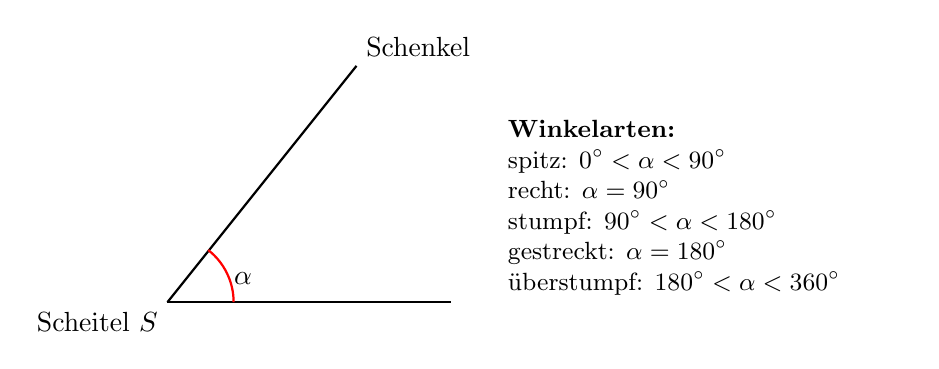
\begin{tikzpicture}[scale=1.2]
  % Scheitelpunkt
  \coordinate (O) at (0,0);
  % Schenkel
  \coordinate (A) at (3,0);
  \coordinate (B) at (2,2.5);
  \draw[thick] (O) -- (A);
  \draw[thick] (O) -- (B);
  % Winkelbogen
  \draw[thick, red] (0.7,0) arc (0:52:0.7);
  \node at (0.8,0.25) {$\alpha$};
  % Beschriftungen
  \node[below right] at (A) {};
  \node[above right] at (B) {Schenkel};
  \node[below left] at (O) {Scheitel $S$};
  % Erklärungen
  \node[right] at (3.5,1) {\parbox{5cm}{
    \small 
    \textbf{Winkelarten:}\\
    spitz: $0^\circ < \alpha < 90^\circ$\\
    recht: $\alpha = 90^\circ$\\
    stumpf: $90^\circ < \alpha < 180^\circ$\\
    gestreckt: $\alpha = 180^\circ$\\
    überstumpf: $180^\circ < \alpha < 360^\circ$
  }};
\end{tikzpicture}
\end{center}

\textbf{Gut zu wissen:}
\begin{itemize}
    \item Wir bezeichnen Winkel meist mit griechischen Buchstaben: $\alpha$ (Alpha), $\beta$ (Beta), $\gamma$ (Gamma)
    \item Ein voller Kreis hat $360^\circ$, ein rechter Winkel $90^\circ$, ein gestreckter Winkel $180^\circ$
    \item Mit dem Geodreieck können wir Winkel messen und zeichnen
\end{itemize}

\subsection*{2. Abbildungen in der Geometrie}

Eine geometrische Abbildung verändert die Position einer Figur. Die wichtigsten Abbildungen sind:

\subsubsection*{a) Punktspiegelung}

\begin{center}
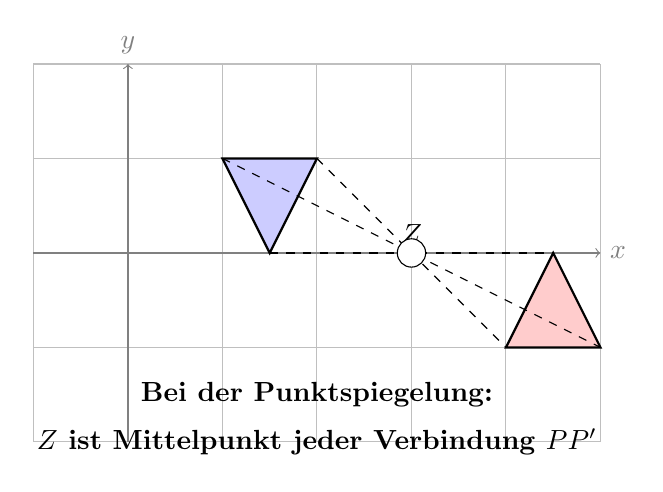
\begin{tikzpicture}[scale=1.2]
  % Koordinatensystem
  \draw[thin,gray!50] (-1,-2) grid (5,2);
  \draw[->,gray] (-1,0) -- (5,0) node[right] {$x$};
  \draw[->,gray] (0,-2) -- (0,2) node[above] {$y$};
  
  % Figur (Dreieck)
  \coordinate (A) at (1,1);
  \coordinate (B) at (2,1);
  \coordinate (C) at (1.5,0);
  \draw[thick, fill=blue!20] (A) -- (B) -- (C) -- cycle;
  
  % Spiegelpunkt
  \coordinate (Z) at (3,0);
  \fill (Z) circle (2pt) node[above] {$Z$};
  
  % Gespiegelte Figur
  \coordinate (A') at (5,-1);
  \coordinate (B') at (4,-1);
  \coordinate (C') at (4.5,0);
  \draw[thick, fill=red!20] (A') -- (B') -- (C') -- cycle;
  
  % Verbindungslinien
  \draw[dashed] (A) -- (A');
  \draw[dashed] (B) -- (B');
  \draw[dashed] (C) -- (C');
  
  % Markierung Mittelpunkt
  \draw[fill=white] (Z) circle (0.15);
  
  % Erklärungen
  \node at (2,-1.5) {\textbf{Bei der Punktspiegelung:}};
  \node at (2,-2) {\textbf{$Z$ ist Mittelpunkt jeder Verbindung $PP'$}};
\end{tikzpicture}
\end{center}

\textbf{Merke:}
\begin{itemize}
    \item Bei der Punktspiegelung wird jeder Punkt $P$ an einem Spiegelpunkt $Z$ gespiegelt
    \item Der Bildpunkt $P'$ liegt auf der Verlängerung der Strecke $PZ$ mit $|PZ| = |ZP'|$
    \item Die Form und Größe bleiben erhalten, aber die Figur wird um $180^\circ$ gedreht
\end{itemize}

\subsubsection*{b) Achsenspiegelung}

\begin{center}
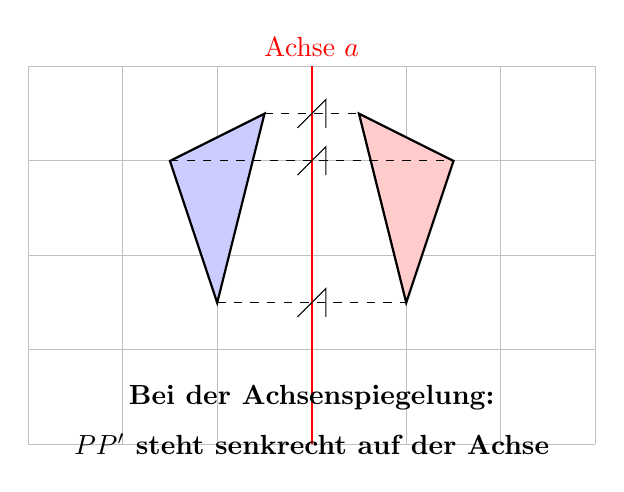
\begin{tikzpicture}[scale=1.2]
  % Koordinatensystem
  \draw[thin,gray!50] (-1,-2) grid (5,2);
  
  % Spiegelachse
  \draw[thick,red] (2,-2) -- (2,2) node[above] {Achse $a$};
  
  % Original Figur (Dreieck)
  \coordinate (A) at (0.5,1);
  \coordinate (B) at (1.5,1.5);
  \coordinate (C) at (1,-0.5);
  \draw[thick, fill=blue!20] (A) -- (B) -- (C) -- cycle;
  
  % Gespiegelte Figur
  \coordinate (A') at (3.5,1);
  \coordinate (B') at (2.5,1.5);
  \coordinate (C') at (3,-0.5);
  \draw[thick, fill=red!20] (A') -- (B') -- (C') -- cycle;
  
  % Verbindungslinien und Lot
  \draw[dashed] (A) -- (A');
  \draw[dashed] (B) -- (B');
  \draw[dashed] (C) -- (C');
  
  % Rechte Winkel markieren
  \draw (2,1) +(-0.15,-0.15) -- +(0.15,0.15) -- +(0.15,-0.15);
  \draw (2,1.5) +(-0.15,-0.15) -- +(0.15,0.15) -- +(0.15,-0.15);
  \draw (2,-0.5) +(-0.15,-0.15) -- +(0.15,0.15) -- +(0.15,-0.15);
  
  % Erklärung
  \node at (2,-1.5) {\textbf{Bei der Achsenspiegelung:}};
  \node at (2,-2) {\textbf{$PP'$ steht senkrecht auf der Achse}};
\end{tikzpicture}
\end{center}

\textbf{Merke:}
\begin{itemize}
    \item Bei der Achsenspiegelung wird jeder Punkt $P$ an einer Achse $a$ gespiegelt
    \item Die Verbindungslinie $PP'$ steht senkrecht auf der Spiegelachse
    \item Der Abstand von $P$ zur Achse ist gleich dem Abstand von $P'$ zur Achse
\end{itemize}

\subsubsection*{c) Verschiebung (Translation)}

\begin{center}
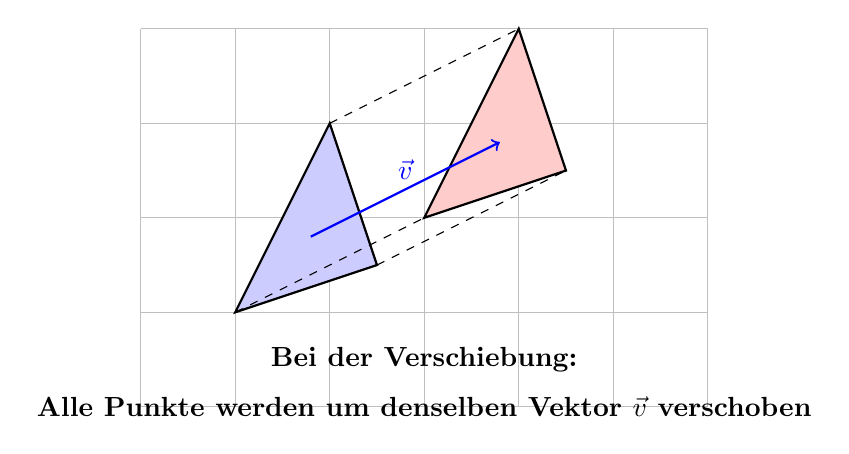
\begin{tikzpicture}[scale=1.2]
  % Koordinatensystem
  \draw[thin,gray!50] (-1,-1) grid (5,3);
  
  % Original Figur (Dreieck)
  \coordinate (A) at (0,0);
  \coordinate (B) at (1,2);
  \coordinate (C) at (1.5,0.5);
  \draw[thick, fill=blue!20] (A) -- (B) -- (C) -- cycle;
  
  % Verschobene Figur
  \coordinate (A') at (2,1);
  \coordinate (B') at (3,3);
  \coordinate (C') at (3.5,1.5);
  \draw[thick, fill=red!20] (A') -- (B') -- (C') -- cycle;
  
  % Verschiebungsvektor
  \draw[->,thick,blue] (0.8,0.8) -- (2.8,1.8) node[midway, above] {$\vec{v}$};
  
  % Verbindungslinien
  \draw[dashed] (A) -- (A');
  \draw[dashed] (B) -- (B');
  \draw[dashed] (C) -- (C');
  
  % Erklärung
  \node at (2,-0.5) {\textbf{Bei der Verschiebung:}};
  \node at (2,-1) {\textbf{Alle Punkte werden um denselben Vektor $\vec{v}$ verschoben}};
\end{tikzpicture}
\end{center}

\textbf{Merke:}
\begin{itemize}
    \item Bei der Verschiebung (Translation) werden alle Punkte um denselben Vektor $\vec{v}$ verschoben
    \item Der Vektor gibt Richtung und Länge der Verschiebung an
    \item Form und Größe der Figur bleiben unverändert
\end{itemize}

\subsection*{Was passiert mit Dreiecken bei diesen Abbildungen?}

\begin{center}
\begin{tabular}{|p{4cm}|p{4cm}|p{4cm}|}
\hline
\textbf{Punktspiegelung} & \textbf{Achsenspiegelung} & \textbf{Verschiebung} \\
\hline
Form und Größe bleiben erhalten & Form und Größe bleiben erhalten & Form und Größe bleiben erhalten \\
\hline
Orientierung wird umgekehrt & Orientierung wird umgekehrt & Orientierung bleibt erhalten \\
\hline
$\Delta ABC \to \Delta A'B'C'$ & $\Delta ABC \to \Delta A'B'C'$ & $\Delta ABC \to \Delta A'B'C'$ \\
\hline
\end{tabular}
\end{center}

\textbf{Tipp zum Üben:} Zeichne ein Dreieck auf kariertes Papier und probiere selbst verschiedene Abbildungen aus!

\section*{Dreiecke und ihre Eigenschaften}

\subsection*{1. Dreieckssorten nach Winkeln}

%\begin{center}
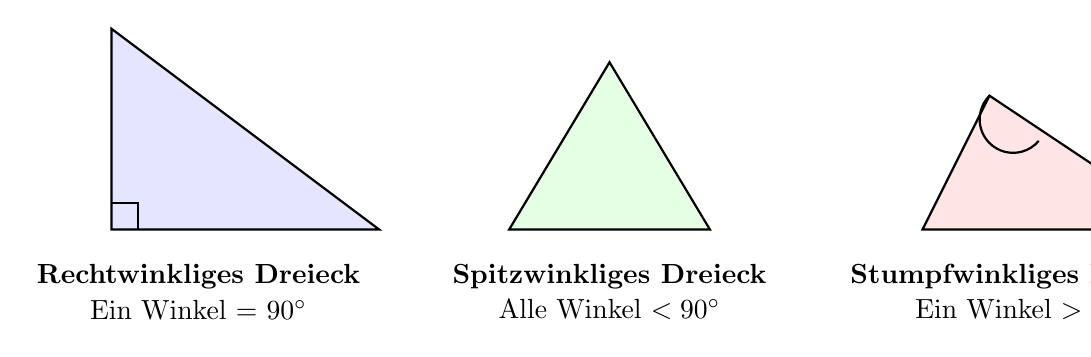
\begin{tikzpicture}[scale=0.85]
  % Rechtwinkeliges Dreieck
  \begin{scope}[shift={(-5,0)}]
    \coordinate (A) at (0,0);
    \coordinate (B) at (4,0);
    \coordinate (C) at (0,3);
    \draw[thick, fill=blue!10] (A) -- (B) -- (C) -- cycle;
    % Rechter Winkel markieren
    \draw[thick] (0.4,0) -- (0.4,0.4) -- (0,0.4);
    \node at (1.3,-0.7) {\textbf{Rechtwinkliges Dreieck}};
    \node at (1.3,-1.2) {Ein Winkel = $90^\circ$};
  \end{scope}
\hspace{.8cm}
  % Spitzwinkliges Dreieck
  \begin{scope}[shift={(0,0)}]
    \coordinate (A) at (0,0);
    \coordinate (B) at (3,0);
    \coordinate (C) at (1.5,2.5);
    \draw[thick, fill=green!10] (A) -- (B) -- (C) -- cycle;
    \node at (1.5,-0.7) {\textbf{Spitzwinkliges Dreieck}};
    \node at (1.5,-1.2) {Alle Winkel $< 90^\circ$};
  \end{scope}
\hspace{1cm}
  % Stumpfwinkliges Dreieck
  \begin{scope}[shift={(5,0)}]
    \coordinate (A) at (0,0);
    \coordinate (B) at (4,0);
    \coordinate (C) at (1,2);
    \draw[thick, fill=red!10] (A) -- (B) -- (C) -- cycle;
    \node at (1.5,-0.7) {\textbf{Stumpfwinkliges Dreieck}};
    \node at (1.5,-1.2) {Ein Winkel $> 90^\circ$};
    % Stumpfer Winkel
    \draw[thick] (1,2) +(0,0) arc (135:320:0.5);
  \end{scope}
\end{tikzpicture}
%\end{center}

\subsection*{2. Dreieckssorten nach Seitenlängen}

\begin{center}
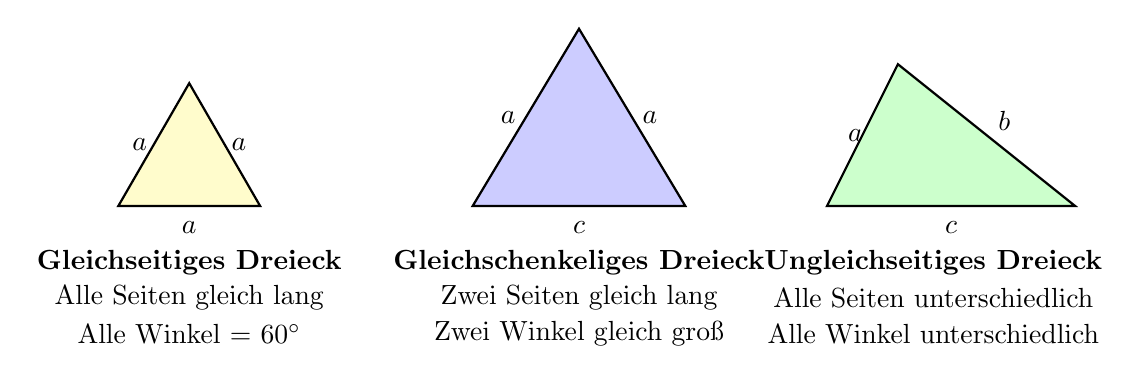
\begin{tikzpicture}[scale=0.9]
  % Gleichseitiges Dreieck
  \begin{scope}[shift={(-5,0)}]
    \coordinate (A) at (0,0);
    \coordinate (B) at (2,0);
    \coordinate (C) at (1,1.732);
    \draw[thick, fill=yellow!20] (A) -- (B) -- (C) -- cycle;
    % Seiten beschriften
    \node at (1,-0.3) {$a$};
    \node at (1.7,0.866) {$a$};
    \node at (0.3,0.866) {$a$};
    \node at (1,-0.8) {\textbf{Gleichseitiges Dreieck}};
    \node at (1,-1.3) {Alle Seiten gleich lang};
    \node at (1,-1.8) {Alle Winkel = $60^\circ$};
  \end{scope}

  % Gleichschenkeliges Dreieck
  \begin{scope}[shift={(0,0)}]
    \coordinate (A) at (0,0);
    \coordinate (B) at (3,0);
    \coordinate (C) at (1.5,2.5);
    \draw[thick, fill=blue!20] (A) -- (B) -- (C) -- cycle;
    % Seiten beschriften
    \node at (1.5,-0.3) {$c$};
    \node at (2.5,1.25) {$a$};
    \node at (0.5,1.25) {$a$};
    \node at (1.5,-0.8) {\textbf{Gleichschenkeliges Dreieck}};
    \node at (1.5,-1.3) {Zwei Seiten gleich lang};
    \node at (1.5,-1.8) {Zwei Winkel gleich groß};
  \end{scope}

  % Ungleichseitiges Dreieck
  \begin{scope}[shift={(5,0)}]
    \coordinate (A) at (0,0);
    \coordinate (B) at (3.5,0);
    \coordinate (C) at (1,2);
    \draw[thick, fill=green!20] (A) -- (B) -- (C) -- cycle;
    % Seiten beschriften
    \node at (1.75,-0.3) {$c$};
    \node at (2.5,1.2) {$b$};
    \node at (0.4,1) {$a$};
    \node at (1.5,-0.8) {\textbf{Ungleichseitiges Dreieck}};
    \node at (1.5,-1.3) {Alle Seiten unterschiedlich};
    \node at (1.5,-1.8) {Alle Winkel unterschiedlich};
  \end{scope}
\end{tikzpicture}
\end{center}

\subsection*{3. Wichtige Formeln für Dreiecke}

\begin{center}
\begin{tabular}{|p{4cm}|p{8cm}|}
\hline
\textbf{Eigenschaft} & \textbf{Formel} \\
\hline
Umfang & $u = a + b + c$ \\
\hline
Flächeninhalt & $A = \frac{1}{2} \cdot g \cdot h$ \\
\hline
Winkelsumme & $\alpha + \beta + \gamma = 180^\circ$ \\
\hline
Satz des Pythagoras & $a^2 + b^2 = c^2$ (im rechtwinkligen Dreieck) \\
\hline
\end{tabular}
\end{center}

\subsection*{4. Besondere Linien im Dreieck}

\begin{center}
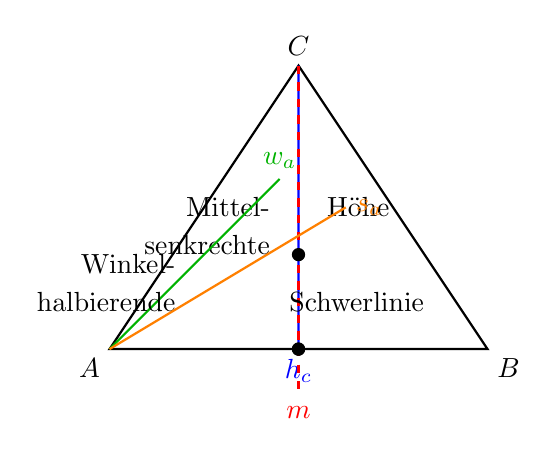
\begin{tikzpicture}[scale=1.2]
  % Grunddreieck
  \coordinate (A) at (0,0);
  \coordinate (B) at (4,0);
  \coordinate (C) at (2,3);
  \draw[thick] (A) -- (B) -- (C) -- cycle;
  
  % Beschriftung der Ecken
  \node[below left] at (A) {$A$};
  \node[below right] at (B) {$B$};
  \node[above] at (C) {$C$};
  
  % Höhe
  \draw[blue, thick] (C) -- (2,0) node[below] {$h_c$};
  \node[right] at (2.2,1.5) {Höhe};
  
  % Mittelsenkrechte
  \draw[red, thick, dashed] (2,3) -- (2,-0.5) node[below] {$m$};
  \fill (2,0) circle (2pt);
  \node[left] at (1.8,1.5) {Mittel-};
  \node[left] at (1.8,1.1) {senkrechte};
  
  % Winkelhalbierende
  \draw[green!70!black, thick] (0,0) -- (1.8,1.8) node[above] {$w_a$};
  \node[left] at (0.8,0.9) {Winkel-};
  \node[left] at (0.8,0.5) {halbierende};
  
  % Schwerlinie
  \fill (2,0) circle (2pt);
  \draw[orange, thick] (A) -- (2.5,1.5) node[right] {$s_a$};
  \fill (2,1) circle (2pt);
  \node[right] at (1.8,0.5) {Schwerlinie};
\end{tikzpicture}
\end{center}

\subsection*{5. Übungsaufgaben}

\begin{enumerate}
  \item Zeichne ein gleichschenkeliges Dreieck mit der Basis $c = 6$ cm und den Schenkeln $a = b = 4$ cm. Konstruiere alle Höhen.
  
  \item Zeichne ein Dreieck $ABC$ mit $AB = 5$ cm, $BC = 4$ cm und dem Winkel bei $B = 60^\circ$. Spiegle es am Punkt $S(3,2)$.
  
  \item Bestimme den Flächeninhalt eines rechtwinkligen Dreiecks mit den Katheten $a = 5$ cm und $b = 12$ cm.
  
  \item Zeichne ein beliebiges Dreieck und konstruiere dessen Mittelsenkrechten. Wo schneiden sie sich?
  
  \item Stelle eine Figur (z.B. ein Haus) aus verschiedenen Dreiecken zusammen und spiegle sie an einer Achse deiner Wahl.
\end{enumerate}




